To evaluate the behavior and accuracy of ConPaaS when hosting web applications, we prepared a realistic and complex enough scenario to assess any PaaS. In particular, we deployed the Wikipedia web application called MediaWiki~\cite{mediawiki}, and used a web hosting benchmark called WikiBench~\cite{wikibench}. 

%In this section, we describe our scenario in detail.

The architecture of the Wikipedia website uses a http-proxy, a http-web server, a database and one or more PhP servers. To deploy the Wikipedia services on ConPaaS, we composed two different services: the PHP web hosting and MySQL service. In the MySQL service, we installed a complete copy of English Wikipedia database which contains about 30GB in Wikipedia articles. In the PhP service, an initial configuration was composed of one Nginx http-proxy, one Apache server, and one or more PhP (FastCGI Process Manager) servers. Each PhP server hosts the MediaWiki application which is the main component of this system. 


\subsection{Characteristics of its workload}

In order to benchmark ConPaaS when hosting the Wikipedia services, we used the WikiBench research tool which generates realistic benchmarks with adaptable traffic properties. WikiBench has a number of advantages compared to the existing benchmark tools for web applications. First of all, Wikibench traces add a high degree of realism, since it is entirely based on the Wikipedia software and data. Indeed, the benchmark workloads are generated based on real access traces from the WikiMedia Foundation. These traces contain detailed  traffic logs of requests made to Wikipedia by its users. Since the original Wikipedia traces can reach peaks of 50000 or 60000 reqs./secs, WikiBench uses the original 10\% sample of these traces which can generate a workload up to about 5000 reqs./secs. As an example, in Figure~\ref{workload}, we show the workload of one trace, named "test", as the number of PhP requests per minute during approximately one day.  In this paper, we focus on the behavior of PhP requests which makes particularly difficult to predict their execution times using auto-scaling sytems. 

Even though we use a 10\% of the real traces, they are very heterogeneous in terms of workload-mix, and thus explaining the irregular performance pattern followed by web applications. To illustrate this heterogeneity, in Figure~\ref{phpRespTimeDispersion}, we present the distribution of the response time values for the PhP requests during the execution of the trace "test". Note that, static provisioning was utilized to execute this trace. A first observation shows an irregular dispersion of the response time values in two levels: (i) a long-term level on which the values vary along the trace execution without following any pattern; and (ii) a short-term level on which the response times widely diverge under short period of time such as one minute. There are two reasons for this dispersion: (i) PhP pages often require database queries; (ii) PhP pages need third-party static files. These issues avoids the utilization of provisioning techniques which scale applications only based on current response values. 

Similarly, as shown in Figure~\ref{workload} and Figure~\ref{phpRespTimeDispersion}, there is not any correlation between the PhP request volumes and their response times. More precisely in Figure~\ref{phpRespTimeDispersion}, the highest response time values obtained in the interval of time 600min. match up with a drop in the request rate during the same interval in Figure~\ref{workload}. Therefore, any provisioning technique that makes decisions based on the request rate can incur errors by under- or over-provisioning an application, which drastically reduces the efficiency of the scaling actions. 

\corina{Are you sure the results from Figures 3 and 4 are relevant? In
figure 3, the response time might be higher for a lower request rate
because there are fewer backend VMs provisioned when the request rate
is low?}

\fixme{ OTHER POSSIBILITY: More precisely in Figure~\ref{reqRate}, the highest response time values obtained during the trace execution, match up with low levels of requests rate. Therefore, ...  }

% Similarly, the intensity of the resulting traffic could also be modified ranging from very low up to the 
% original traffic intensity of the trace. 

%Initial benchmark results show a typical day of Wikipedia traffic and the relation between the request rate %and the server response times. 


\begin{figure}
\begin{center}
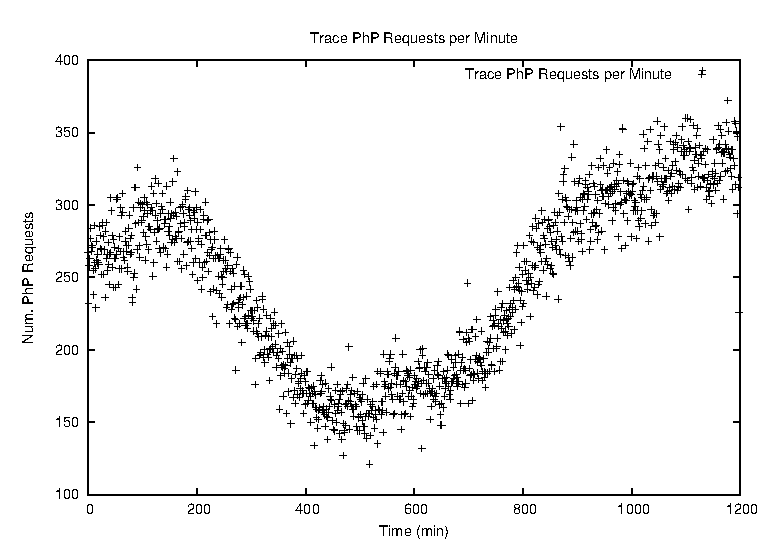
\includegraphics[width=0.49\textwidth, height=6cm]{./images/traceWorkload}
\end{center}
\caption{Wikipedia trace workload}
\label{workload}
\end{figure}

In addition, other properties may be also considered important when using the Wikipedia traces:

\begin{itemize}
\item The intervarrival time between requests follows a Poisson distribution.

\item The distribution of page popularity varies from very popular pages to those being accessed very infrequently.

\item The mix of static/dynamic requests presents a strong variation. 

\begin{figure}
\begin{center}
\includegraphics[width=0.49\textwidth, height=6cm]{./images/phpRespTimeDispersion}
\end{center}
\caption{Complexity of PhP requests}
\label{phpRespTimeDispersion}
\end{figure}

\item The ratio of read/write operations vary having more reads than editions or creations of wiki pages.

\begin{figure}
\begin{center}
\includegraphics[width=0.49\textwidth, height=6cm]{./images/staticProv_reqRate}
\end{center}
\caption{Response time vs request rate}
\label{reqRate}
\end{figure}

\item A considerable amount of requests for non-existing pages and files add realism to the traffic.

\end{itemize}


%By using real world server side software and data, we think the WikiBench benchmarking suite is a very  realistic and extensible research tool.

% these traces create workloads for WikiBench instead of creating purely synthetic workloads like other benchmarking tools have done.

Since Wikipedia has a variable amount of data and visitors, it represents a valid example of elastic web application. In this paper, we focus in the scalability of the PhP web hosting service, and thereby as the number of PhP servers hosting MediaWiki scale out or back based on the demanding workload.

